\documentclass[11pt]{article}
\pagestyle{empty}
%\usepackage[latin1]{inputenc}
\usepackage[utf8]{inputenc}
\usepackage{a4wide}
\usepackage{amsmath}
\usepackage{amssymb}
\usepackage{amsthm}
\usepackage{german}
\usepackage{multirow,array}
\usepackage{hyperref}
 \usepackage{graphicx}
%\usepackage{ipe}
%\input{thmstyle-ger}

\parindent0mm
\sloppy

% Basic data
\newcommand{\VORLESUNG}{Induktive Statistik für Soziologinnen und Soziologen}
\newcommand{\STAFF}{Mariana Nold}
\newcommand{\ASSIGNMENT}{1}
\newcommand{\HANDOUT}{Montag, den 23.Oktober   2017}
\newcommand{\DELIVER}{Freitag 10. November 2017}
\newcommand{\PRACTICAL}[1]{\marginpar{\tiny {\bf Aufgabe \\ abgeben!} #1}}
\newcommand{\FAUFTRAG}[1]{\marginpar{\tiny {\bf selbst entdeckendes Verstehen} #1}}
\newcommand{\titel}{Zufallsvorgang, Inferenzschluss und Wahrscheinlichkeitsverteilungen}
\newcommand{\startwert}{0}

% Arbitrary packages and settings

\newcommand{\N}{\mathbb{N}}
\newcommand{\floor}[1]{\lfloor{#1}\rfloor}
\newcommand{\ceil}[1]{\lceil{#1}\rceil}
\newcommand{\half}[1]{\frac{#1}{2}}
\newcommand{\punkte}[1]{{\small{ }(#1 Punkte)}}
\newcommand{\punkt}[1]{{\small{ }(#1 Punkt)}}

\newcommand{\aufgabe}[1]{\item{\bf #1}}
\newcommand{\hinweis}{{\em Hinweis}}

\begin{document}
% Document title

\begin{center}
\ASSIGNMENT{}. Aufgabenblatt vom \HANDOUT{} zur Vorlesung 
\vspace*{0.5cm}

{\Large \VORLESUNG{}}
%\PRACTICAL{}
(\STAFF{}) 


\vspace*{0.5cm}
{\textbf{Thema:} \titel{}\\}
\vspace*{0.2cm}

{\small Abgabe: \DELIVER{}}
\vspace*{1cm}
\end{center}

Wichtige Definitionen und Begriffe aus den ersten beiden Vorlesungen:
\begin{itemize}
\item{Zufallsvorgang}
\item{Zufallsvariable}
\item{Einfache Zufallsstichprobe}
\item{Wahrscheinlichkeitsverteilung}
\item{Binäre Variable und  Bernoulliverteilung}
\item{Binomialverteilung}
\end{itemize}
%\vspace{2cm}
\begin{enumerate}\addtocounter{enumi}{\startwert}



\aufgabe{Verteilung des Taschengeldes beschreiben}\\ \punkte{18}  \PRACTICAL{}\\
Der Datensatz \texttt{taschengeld.dta} enthält die Ergebnisse einer fiktiven 
Befragung von $100$ Grundschulkindern aus Jena zu folgenden Merkmalen:
\begin{itemize}
\item{id: Zahl zwischen $1$ und $100$ zur Identifizierung der Person}
\item{TG: monatliches Taschengeld in Euro}
\item{G: Geschlecht ($0:$ Junge, $1:$ Mädchen)}
\item{WSp: Antwort auf die Frage, ob Wassersport zu den drei Lieblingssparorten gehört 
($0:$ nein, $1:$ ja)}
\end{itemize}

% http://www.psychstatistics.com/2011/05/30/stata-descriptive-statistics-mean-median-variability/

% https://www.karteikarte.com/lesson/83164/statistik-1
% https://www.cobocards.com/pool/de/card/3zc520512/online-karteikarten-statistik-was-ist-ein-inferenzschluss-/
 \begin{enumerate}
 \item{Nennen Sie für jedes der vier Merkmale das Messniveau.}\\ \punkte{4}
 \item{Nutzen Sie die Übersichtstabellen der 1. Vorlesung um geeignete Lage- und Streuungsmaße
 zur Beschreibung des Merkmals TG auszuwählen.\\ Berechnen Sie diese Maße und interpretieren Sie sie inhaltlich.\\
 Nutzen Sie den \texttt{STATA}-Befehl \\ \texttt{. summarize TG}.}\\ \punkte{4}
 \item{ Ein Inferenzschluss ist der Rückschluss von Eigenschaften einer Stichprobe auf Eigenschaften einer Grundgesamtheit, wobei man die Irrtumswahrscheinlichkeit angeben kann. Nehmen Sie an, ihre Hypothese lautet: ``Der Mittelwert des Taschengeldes von Grundschulkindern in Jena ist höher als $11$ Euro.''\\ Welche
 zwei Möglichkeiten gibt es, beim Inferenzschluss einen Fehler zu machen?}\\ \punkte{2}
 \item{Nutzen Sie den \texttt{STATA}-Befehl \\ \texttt{. graph box TG, over(G)}\\ um den Boxplots
 der Jungs und den Boxplot der Mädchen zu vergleichen. \\Fassen Sie ihren Eindruck mit Bezug
 auf die Quartile in zwei bis drei Sätzen zusammen.
 Nutzen Sie für ihre Beschreibung den \texttt{STATA}-Befehl: \\ \texttt{. bysort G: summarize TG, detail}\\ um die Zahlenwerte
 der Quartile zu erfahren.}\\ \punkte{4}
 \item{Als Modellverteilung zur Approximation der empirischen Verteilung der Taschengeldes
 wir die Normalverteilung mit $\hat{\mu}=12.35$ und $\hat{\sigma}=2.71$ verwendet.
 Die Abbildungen \ref{abb1}  zeigt die Dichte und Verteilungsfunktion. In welcher Beziehung 
 stehen die beiden Funktionen? Antworten Sie in zwei bis drei Sätzen.}\\ \punkte{4}
 %\newpage
  \begin{figure}[ht]
 	\centering
 	      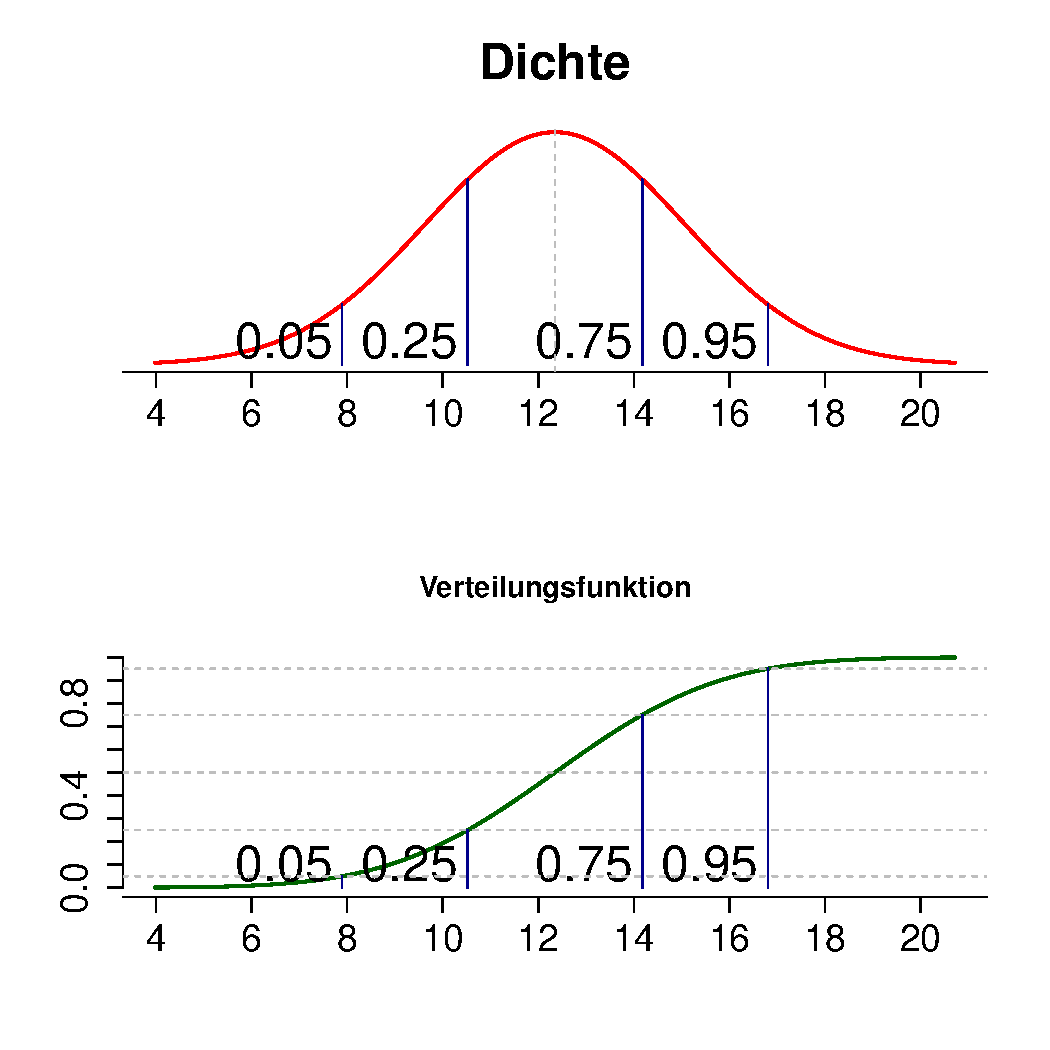
\includegraphics[width=0.80\textwidth]{both.pdf}
 	      \caption{Dichte und Verteilungsfunktion der Normalverteilung
 	       \label{abb1}}
 	\end{figure}
 	
% 	  \begin{figure}[ht]
% 	\centering
% 	      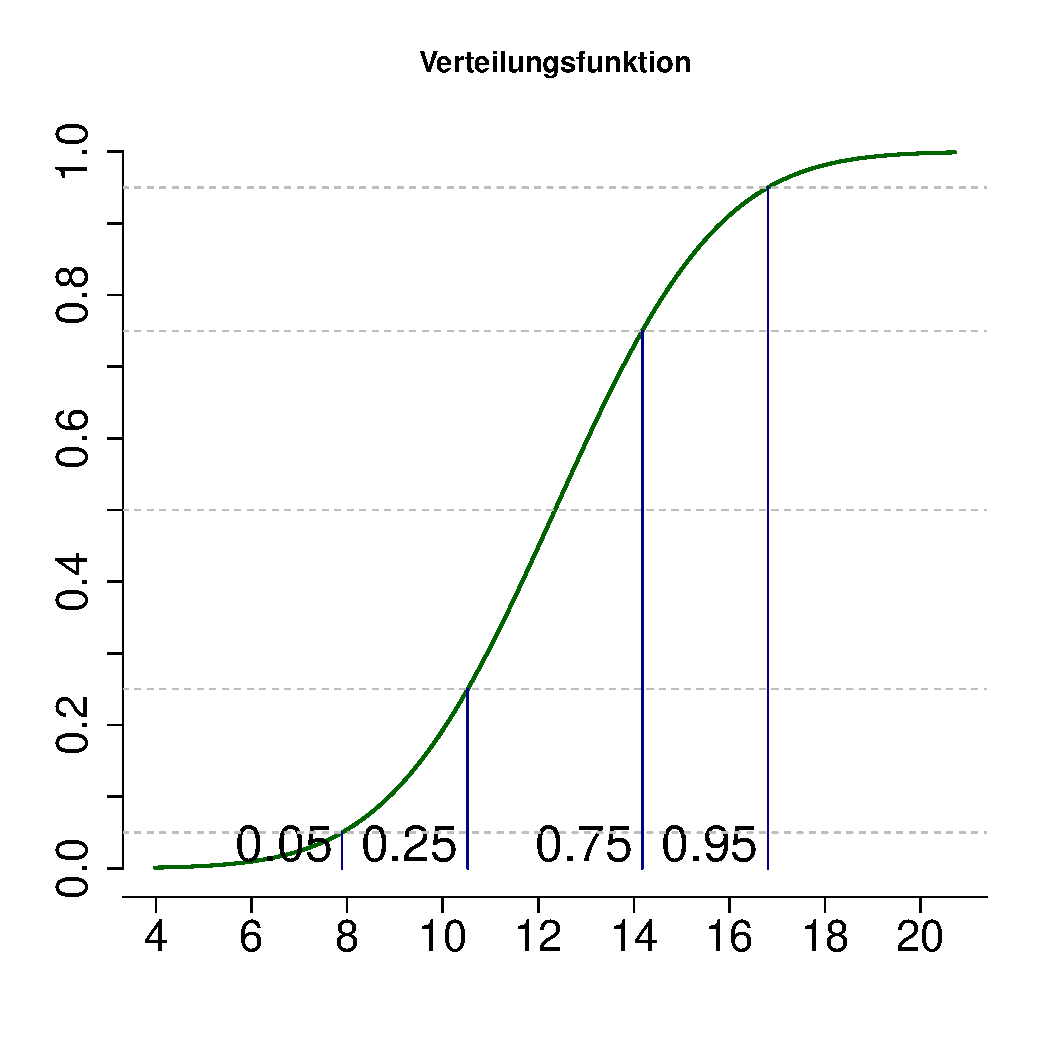
\includegraphics[width=0.50\textwidth]{normCDF_TG.pdf}
% 	      \caption{Verteilungsfunktion der Normalverteilung
% 	       \label{abb2}}
% 	\end{figure}
\end{enumerate}
% https://www.ssc.wisc.edu/sscc/pubs/sfs/sfs-ttest.htm
%  ttest TG, by(G)
\newpage
\aufgabe{Wiederholung: Prozentsatzdifferenz  in $2 \times 2$-Kreuztabellen}\\
 (siehe Übungsblatt 5, Aufgabe 19 aus dem letzten Semester)\\
Sie sollen die Antwort auf die Frage, ob Wassersport zu den drei Lieblingssparorten gehört 
(WSP $0:$ nein, $1:$ ja), als abhängige Variable auffassen und das Geschlecht (G $0:$ Junge $1:$ Mädchen).
Im Folgenden wird die unabhängige Variable mit $X$ und die abhängige Variable mit $Y$ bezeichnet.

%   \begin{table}[h]
%  \centering
%    \setlength{\extrarowheight}{2pt}
%    \begin{tabular}{cc|c|c|}
%      & \multicolumn{1}{c}{} & \multicolumn{2}{c}{ $X$}\\
%      & \multicolumn{1}{c}{} & \multicolumn{1}{c}{$0$}  & \multicolumn{1}{c}{$1$} \\\cline{3-4}
%      \multirow{2}*{ $Y$}  & $0$ & $h_{1,1}$ & $h_{1,2}$ \\\cline{3-4}
%      & $1$ &  $h_{2,1}$ &  $h_{2,2}$ \\\cline{3-4}
%    \end{tabular}
%   % \caption{ \label{tab2by2}}
%  \end{table}

   \begin{table}[h]
  \centering
    \setlength{\extrarowheight}{2pt}
    \begin{tabular}{cc|c|c|c}
      & \multicolumn{1}{c}{} & \multicolumn{2}{c}{ $X$}\\
      & \multicolumn{1}{c}{} & \multicolumn{1}{c}{Junge}  & \multicolumn{1}{c}{Mädchen} & \multicolumn{1}{c}{$\sum$}\\\cline{3-4}
      \multirow{2}*{ $Y$}  & nein & $h_{1,1}$ & $h_{1,2}$ &$h_{1,\bullet}$ \\\cline{3-4}
      & ja &  $h_{2,1}$ &  $h_{2,2}$ & $ h_{2,\bullet}$ \\\cline{3-4}
     & \multicolumn{1}{c}{$\sum$ } & \multicolumn{1}{c}{$h_{\bullet,1}$}  & \multicolumn{1}{c}{$ h_{\bullet,2}$} & \multicolumn{1}{c}{}
    \end{tabular}
    \caption{ \label{tab2by2}$2 \times 2$-Kreuztabelle für die Merkmale Geschlecht (X) und Lieblingssportart Wassersport (Y)}
  \end{table}
\begin{enumerate}
\item{Gemäß der in den Sozialwissenschaften üblichen Konvention: Welcher der beiden folgenden \texttt{STATA}-Befehle
erzeugt, die richtige Tabelle? \\ \texttt{. tab G WSp} oder \texttt{. tab  WSp G} \\
Schreiben Sie Tabelle in Analogie zur Tabelle \ref{tab2by2} mit Zahlenwerten gefüllt auf.}
\item{Berechnen Sie die bedingte relative Häufigkeit (= bedingte Anteilswerte) von $Y|X$ und interpretieren Sie das 
Ergebnis.\\ (Nutzen Sie dazu entweder den \texttt{STATA}-Befehl \texttt{. tab WSp G, col nofreq} oder
tab  G WSp, col nofreq).}
\item{Berechnen und interpretieren  Sie die Prozentsatzdifferenz (bei spaltenbezogener Prozentuierung).
Die Prozentsatzdifferenz (bei spaltenbezogener Prozentuierung) ist definiert als:
$$d_{Y|X} = 100 \cdot \bigg( \frac{h_{1,1}}{h_{\bullet,1}}-\frac{h_{1,2}}{h_{\bullet,2}}\bigg)$$ }
\item{Berechnen Sie mit Hilfe des \texttt{STATA}-Befehl\\ \texttt{. tab WSp G, chi2}\\ den $\chi^{2}$-Koeffizienten
und erklären Sie die inwiefern der $\chi^{2}$-Koeffizienten die bei Unabhängigkeit erwarteten und die tatsächlichen beobachteten
Häufigkeiten vergleicht.}
\end{enumerate}



\aufgabe{Zentrale Definitionen }\\ \punkte{10}  \PRACTICAL{}\\
\begin{enumerate}
\item{Nennen Sie die Definition des Zufallsvorgangs und geben Sie ein Beispiel dazu an.}\\ \punkte{2}
\item{Mit Bezug auf Ihr Beispiel in Teilaufgabe a): Wie lautet die entsprechende Zufallsvariable?}\\ \punkte{2}
\item{Nennen Sie die Definition der binären Variable und geben Sie ein Beispiel dazu an.}\\ \punkte{2}
\item{Suchen Sie ein Beispiel für einen realen Prozess, den man mit Hilfe der Binomialverteilung
modellieren kann. Begründen Sie ihre Auswahl in zwei Sätzen.}\\ \punkte{4}
%\item{}
\end{enumerate}

\end{enumerate}
\end{document}
